% !TEX TS-program = xelatex
% !TEX encoding = UTF-8 Unicode

% In Class Activity for ME3001- Tristan Hill 
% Spring 2017 - Fall 2017 - Fall 2020 - Fall 2021
% Mechanical Engineering Analysis with MATLAB  and Solidworks
% Module 1 - Deisgn with Solidworks
% Activity 2 -(In-Class)- Introduction to Solidworks 

\documentclass[12pt]{article}
\usepackage{/home/thill/Documents/lectures/analysis_lectures/analysis_activities}

% Title and Misc
\newcommand{\COURNAME}{ME 3001-002}
\newcommand{\CURRTERM}{Fall 2021} %Current Term
\newcommand{\MNUM}{1} %Module Number
\newcommand{\ANUM}{3} %Activity Number
\newcommand{\moduletitle}{Non-Linear Equationsw}
\newcommand{\activitytitle}{Mechanical Design Problem} %Module Name
\pagestyle{myheadings}
%\markright{{\large ME4140 - ROS Workshop - \CURRTERM}}

\textwidth=7.0in
\topmargin=-0.6in
\leftmargin=0.5in
\textheight=9.25in
\hoffset=-0.5in
\footskip=0.2in

\begin{document}

\thispagestyle{plain}

\begin{center}
   {\bf \Large In-Class Activity\hspc\ANUM\hspc - \activitytitle}\vspace{3mm}\\
   {\bf \large \COURNAME - Mechanical Engineering Analysis - \CURRTERM} \vspace{5mm}\\
\end{center}

\begin{description}


\item[\textbf{\underline{Learning Objectives:}}] \hfill \vspace{0mm}

\begin{itemize}
	\item Practice using root find methods in MATLAB to solve an applied engineering problem.
\end{itemize}


\item[\textbf{\underline{Overview:}}] \hfill \vspace{3mm}\\

As an engineer you are asked to design a structure. The geometry of this structures is simple but certain properties are critical. 

\item[\textbf{\underline{Overview:}}] \hfill \vspace{3mm}\\
	
	What is the {\it mathematical model} of the cone?  
	
	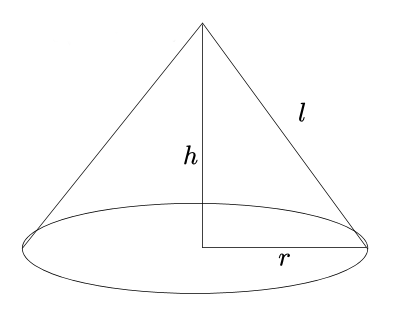
\includegraphics[scale=.35]{lecture3_fig1.png}\\
	\scalebox{1.2}{surface area, $s=\pi r l = \pi r \sqrt{h^2+r^2}$} \\
	\scalebox{1.2}{volume, $v=\pi r^2 \frac{h}{3}$} \\
	
\item[\textbf{\underline{Design Requirements:}}] \hfill \vspace{0mm}

	The design is required be cone with a surface area of exactly $25 m^2$ to a tolerance of 0.1 $m^2$ and a height of exactly $1 m$. Your goal is to find the radius in meters that would produce this exact design.\\
	
\item[\textbf{\underline{Required Materials:}}] \hfill \vspace{0mm}

\begin{itemize}
	\item {\bf Your Computer}: This activity requires a computer with MATLAB installed.
\end{itemize}

\newpage

\item[\textbf{\underline{Activity:}}] \hfill \vspace{0mm}

\begin{enumerate}
	

	\item Write a MATLAB program to solve the mechanical design problem described on the previous page. {\it Remember to put a proper header at the top of your main program, and clear the workspace in the script directly below the header. } The main file of your program should be called {\bf \BL<USERNAME>\BK\_activity\ANUM.sldprt}
	
	\item Test your program with a range of initial guesses for the design variable $r$. Is the algorithm robust to different inputs? 
	
	\item Show the results of your algorithm using three different initial guesses. You can use the default output to the command window the {\it fprintf()} function. Summarize the results in a file {\bf \BL<USERNAME>\BK\_activity\ANUM.pdf }
	
	\item Write a description of how your algorithm works to solve the problem. This can be a few sentences or a bulleted list.
	
	
\end{enumerate}

\item[\textbf{\underline{Submit:}}] \hfill \vspace{0mm}

		Submit the most complete version of {\bf \BL<USERNAME>\BK\_part1.sldprt} \\and {\bf \BL<USERNAME>\BK\_part1.pdf } to the Activity \ANUM \hspace{1mm} folder before the posted due date.

\end{description}
\end{document}
